% Template per la presentazione di laurea
%
% Creato da Giulio Spinozzi
% giuliospinozzi@gmail.com
% http://giuliospinozzi.altervista.org
%
%\makeatletter\let\ifGm@compatii\relax\makeatother %per un bug corrente, da togliere successivamente
\documentclass[12pt, hyperref={bookmarksnumbered=true}]{beamer} %Classe documento, font, segnalibri
\let\Tiny=\tiny	%Ridimensionamento del font, per un corretto rendering
\usepackage{greenAmsterdam}	%Carica il tema
\usepackage{color}	%Per usare colori aggiuntivi
\setbeamercovered{transparent}	%Effetto trasparente delle scritte
%\pgfdeclareimage[height=1.5cm]{logo}{img/logo.png}
\usepackage[latin1]{inputenc}

\title{Generazione automatica di word cloud dinamiche}
%\titlegraphic{\pgfuseimage{logo}}
\subtitle{Ingegneria Informatica e dell'Automazione \vspace{0.5cm}
\\\textsc{\textcolor[rgb]{0.00,0.00,0.00} {Universit� degli Studi di Perugia \\Facolt� di Ingegneria}}}
\author{\textbf{Candidato}: \textit{Enrico Spataro} \hspace{0.1cm} \\\textbf{Relatore}: \textit{Prof.ssa Carla Binucci} \hspace{0.2cm} \\
\textbf{Correlatore}: \textit{Prof. Walter Didimo}}
\date{\scriptsize 19.02.2016}

\begin{document}

\frame{\titlepage}	%Ogni slide � racchiusa dal tag frame

\section[Sommario]{}
\frame{
\frametitle{\textbf{Contenuti}}
\tableofcontents
}


\section{Introduzione}
\frame{
\frametitle{\textbf{Obiettivi}}
\begin{beamerboxesrounded}{}
Mostrare l'evoluzione di un testo tramite:
\begin{itemize}
\item creazione word cloud semantiche ad intervalli regolari;
\item animazioni tramite morphing.
\end{itemize}
\end{beamerboxesrounded}
}

\frame{
\frametitle{\textbf{Cos'� una word cloud?}}
\begin{center}
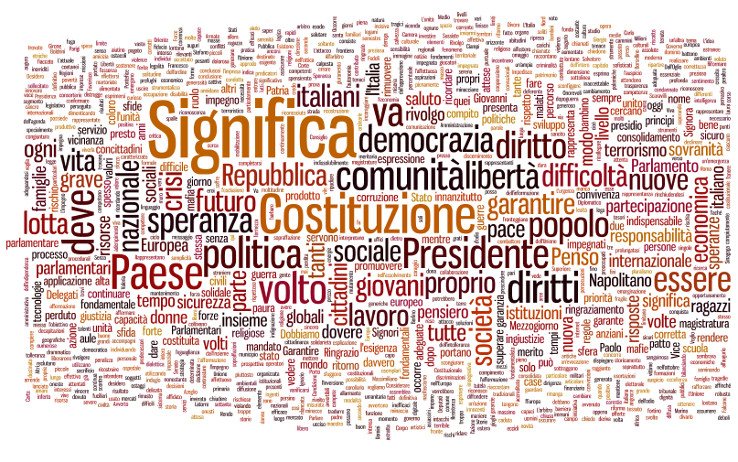
\includegraphics[scale=0.4]{img/wc_statiche/mattarella_wc.png}
\end{center}
}

\frame{
\frametitle{\textbf{Word cloud semantiche}}
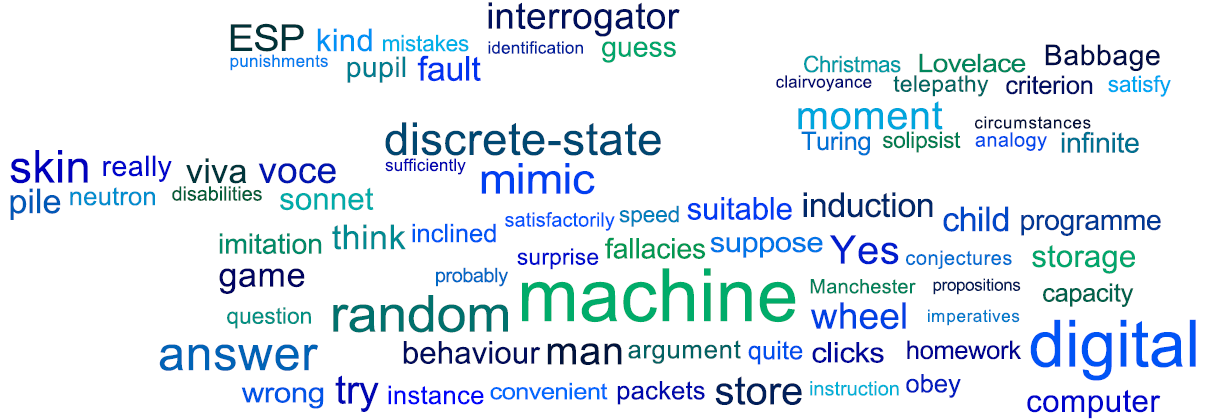
\includegraphics[scale=0.45]{img/wc_statiche/wc_semantic.png}
}

\frame{
\frametitle{\textbf{Word cloud dinamiche}}
\begin{center}
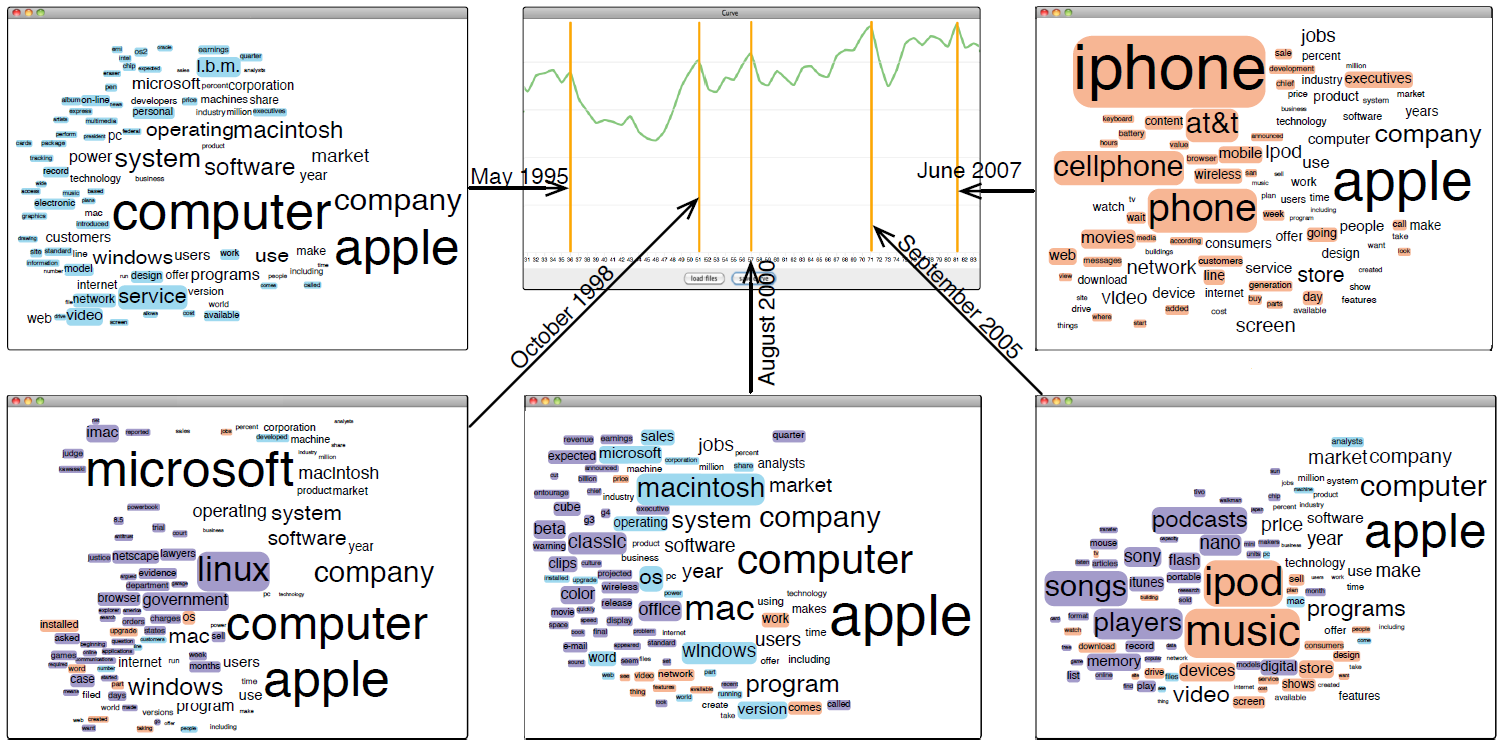
\includegraphics[scale=0.35]{img/wc_dinamiche/cui.png}
\end{center}
}
\frame{
\frametitle{\textbf{Morphing}}
\begin{center}
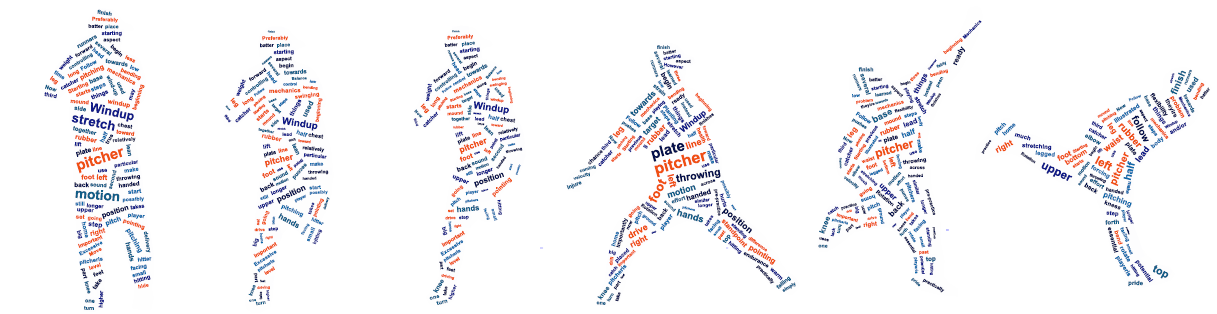
\includegraphics[scale=0.4]{img/wc_dinamiche/pitcher.png}
\end{center}
}

\section{Creazione word cloud}
\subsection{Word cloud statica}
\frame{
\frametitle{\textbf{Generazione word cloud semantica}}
\begin{beamerboxesrounded}[shadow=true]{}
	\begin{enumerate}
\item Estrazione parole chiave
\item Calcolo similarit�
\item Disegno word cloud
\item Clustering
	\end{enumerate}
\end{beamerboxesrounded}
}

\frame{
\frametitle{\textbf{Generazione word cloud semantica}}
\begin{beamerboxesrounded}[shadow=true]{}
	\begin{enumerate}[<+-| alert@+>]
\item <1| alert@+> Estrazione parole chiave
\item <2| alert@+> Calcolo similarit�
\item <3| alert@+> Disegno word cloud
\item <4| alert@+> Clustering
	\end{enumerate}
\end{beamerboxesrounded}
\begin{center}
\includegraphics<1>[scale=0.45]{img/wc_dinamiche/term_ext.png}
\includegraphics<3>[scale=0.45]{img/wc_dinamiche/layout.png}
\includegraphics<4>[scale=0.45]{img/wc_dinamiche/clustering.png}
\end{center}
}

\subsection{Word cloud dinamica}
\frame {
\frametitle{\textbf{Generazione word cloud dinamica}}
Obiettivo: create $K$ word cloud dal testo, si vuole passare da una word cloud alla successiva in modo graduale tramite tecniche di morphing.
}

\frame {
\frametitle{\textbf{Morphing}}
\begin{beamerboxesrounded}[shadow=true]{Caratteristiche}
	\begin{itemize}
\item Numero di frame
\item Gestione stato delle parole
\item Gestione del colore delle parole
\end{itemize}
\end{beamerboxesrounded}
}

\frame{
\frametitle{\textbf{Stato delle parole}}
Le parole, tra una word cloud e la successiva, possono:
\begin{itemize}
\item<2> scomparire
\item<3> apparire
\item<4> rimanere nel layout (variando posizione)
\end{itemize}
\begin{center}
\includegraphics<3>[scale=0.75]{img/wc_dinamiche/new_word.png}
\includegraphics<2>[scale=0.75]{img/wc_dinamiche/disapp_word.png}
\includegraphics<4>[scale=0.6]{img/wc_dinamiche/morphcommon.png}
\end{center}
}

\frame {
\frametitle{\textbf{Generazione word cloud dinamica}}
\begin{beamerboxesrounded}[shadow=true]{Possibili problematiche}
	\begin{enumerate}
\item Variazione posizione delle parole
\item Variazione dei cluster
	\end{enumerate}
\end{beamerboxesrounded}
}

\frame {
\frametitle{\textbf{Generazione word cloud dinamica}}
\begin{beamerboxesrounded}[shadow=true]{Possibili problematiche}
	\begin{enumerate}[<+-| alert@+>]
\item <1| alert@+> Variazione delle parole
\item <2| alert@+> Variazione cluster
	\end{enumerate}
\end{beamerboxesrounded}
\includegraphics<1>[scale=0.45]{img/wc_dinamiche/layout_mod.png}
}


\frame{
\frametitle{\textbf{Inserire video}}
}

\section{Risultati sperimentali}
\frame{
\frametitle{\textbf{Risultati sperimentali}}
Setup: 
\begin{itemize}
\item $200$ discorsi, lunghezza media $17$ minuti.
\item 4 campionamenti per ogni testo.
\item Parole estratte: $20$,$40$,$60$
\end{itemize}
\begin{beamerboxesrounded}[shadow=true]{Metriche}
	\begin{itemize}
\item Combination metric
	\begin{itemize}
	\item Distortion metric
	\item Coherence metric
	\end{itemize}
\item Space metric
\item Tempo d'esecuzione
\end{itemize}
\end{beamerboxesrounded}
}

\frame{
\frametitle{\textbf{Combination metric}}
\includegraphics<1>[scale=0.27]{img/impl_test/test_tfidf_jaccard/figures/combo_20.png}
\includegraphics<2>[scale=0.27]{img/impl_test/test_tfidf_jaccard/figures/combo_40.png}
\includegraphics<3>[scale=0.27]{img/impl_test/test_tfidf_jaccard/figures/combo_40.png}
\includegraphics<4>[scale=0.27]{img/impl_test/test_lexrank_cosine/figures/combo_20.png}
\includegraphics<5>[scale=0.27]{img/impl_test/test_lexrank_cosine/figures/combo_40.png}
\includegraphics<6>[scale=0.27]{img/impl_test/test_lexrank_cosine/figures/combo_60.png}
}

\frame{
\frametitle{\textbf{Space metric}}
\includegraphics<1>[scale=0.27]{img/impl_test/test_tfidf_jaccard/figures/spacemetric_40.png}
}

\frame{
\frametitle{\textbf{Tempo d'esecuzione}}
\begin{itemize}
\item Configurazione caso peggiore: TFIDF, Jaccard Similarity e Star Forest
\item Configurazione caso migliore: Term Frequency, Cosine Similarity e CPWCV
\end{itemize} 
\tabcolsep=6mm
\resizebox{1\columnwidth}{!}   {
\begin{tabular}{ccc}
\hline
Parole estratte & Caso peggiore & Caso migliore  \\
\hline
$20$ & $2.65$ & $0.77$\\
$40$ & $3.01$ & $0.94$\\
$60$ & $3.66$ & $1.25$\\
\hline
\end{tabular}} 
}

\section{Conclusioni}
\frame{
\frametitle{\textbf{Concludendo...}}
Il lavoro di tesi si \`e articolato nelle seguenti fasi:
\begin{enumerate}
\item Lorem ipsum
\item Lorem ipsum
\item Lorem ipsum
\end{enumerate}
\vspace{0.1cm}
\setbeamercolor{postit}{fg=black,bg=green} %Baloon di colore diverso, senza sfondo
\begin{beamerboxesrounded}[upper=postit ,lower=postut ,shadow=true]{Lorem ipsum:}
\begin{itemize}
\item Lorem ipsum
\item Lorem ipsum
\end{itemize}
\end{beamerboxesrounded}
}

\end{document}
